\documentclass[11pt,a4paper]{article}

\usepackage[latin1]{inputenc}
\usepackage{fullpage}
\usepackage{amsmath}
\usepackage{amssymb}
\usepackage{enumerate}
\usepackage{xcolor}
\usepackage{environ}

\usepackage{graphicx}
\usepackage{todonotes}
\usepackage{caption}
\usepackage{subcaption}

\title{Leren --- Homework 3\\[3mm]\small{Chapter 6-8, Alpaydin}}
\date{Deadline: 23:59, Sunday, December 2nd, 2018}

\begin{document}
\maketitle

This is the fifth week's assignment for Leren.  This assignment covers
chapters 6, 7 \& 8 of Alpaydin. Please take note of the following:

\begin{itemize}
  \item You are expected to hand in your solutions in \LaTeX;
  \item This problem set is an individual assignment;
  \item The deadline for this assignment is Sunday, December 2 at 23:59.
\end{itemize}

\newcommand{\xvec}{\boldsymbol{x}}
\newcommand{\xmat}{\boldsymbol{X}}
\newcommand{\cxmat}{\tilde{\xmat}}
\newcommand{\cxn}{\tilde{\xvec}^{i}}
\newcommand{\xvecn}{\xvec^{i}}
\newcommand{\xvecmean}{\boldsymbol{\mu}}
\newcommand{\zn}{\boldsymbol{z}^i}
\newcommand{\vvec}{\boldsymbol{v}}

\section{Chapter 6: Dimensionality Reduction}
\subsection{Principal Component Analysis (PCA)}
Suppose we have a dataset of $N$ vectors $\{\boldsymbol{x}^i\}_{i=1}^N$ of dimension $D$. We can represent the entire dataset as a $N$ by $D$ matrix $\boldsymbol{X}$ (row $i$ is $\boldsymbol{x}^i$). We wish to project this data onto a lower-dimensional subspace and choose PCA as our technique for dimensionality reduction. Consider the following procedure for PCA:

\begin{itemize}
\item [\textbf{Step 1}] Data preprocessing to get $\cxmat$ from $\boldsymbol{X}$ 
\item [\textbf{Step 2}] Compute the sample covariance $\boldsymbol{C}$ of $\cxmat$, i.e.~compute the (unbiased) estimator of $\boldsymbol{\Sigma}=\mathrm{cov}(\cxmat)$.
\item [\textbf{Step 3}] Solve the eigenvalue problem $\boldsymbol{C} = \boldsymbol{V}\boldsymbol{L}\boldsymbol{V}^T$ (spectral decomposition of $\boldsymbol{C}$), where $\boldsymbol{V}$ is a column matrix of eigenvectors $\vvec_k$ and $\boldsymbol{L}$ is a diagonal matrix of eigenvalues $\lambda_k$, i.e.~$\boldsymbol{L}_{kl}=\lambda_k\delta_{kl}$, where $\delta_{kl}=1$ if $k=l$, otherwise $\delta_{kl}=0$.
\item [\textbf{Step 4}] Pick the $K$ eigenvectors with the $K$ largest eigenvalues $\{\vvec_1,\ldots,\vvec_K\}$.
\item [\textbf{Step 5}] Project data onto $K$-dimensional subspace.
\end{itemize}

Answer the following questions:

\begin{enumerate}[(a)]
\item Let's assume that the variance of each of the $D$ variables is approximately the same such that rescaling the variance is not required. What other data preprocessing step (\textbf{Step 1}) is required for PCA? Provide an expression on how this preprocessing can be done. Hint: you can give the expression for $\cxn$ (i.e.~the $i$-th row of the preprocessed data $\cxmat$).
\item What is the dimensionality of $\boldsymbol{C}$?
\item How do we construct $\boldsymbol{W}$? Reminder: $\boldsymbol{W}$ is the linear projection that maps data vectors $\cxn$ onto the $K$-dimensional principal subspace, i.e.~$\zn=\boldsymbol{W}^T\cxn$.
\item How do we obtain the PCA reconstruction $\boldsymbol{\hat{x}}^i$ of $\boldsymbol{x}^i$ from the projected data point $\zn$? Provide an expression.
\item Consider the three different proposals of principal components  for the same 2-dimensional dataset in Figure~\ref{fig:pca_proposal} (principal components displayed in orange). Identify the true principal components that would be found by applying PCA. For each proposal briefly explain your decision why these are (not) the correct principal components.
    \begin{figure}[ht]
        \centering
        \begin{subfigure}{.33\textwidth}
          \centering
          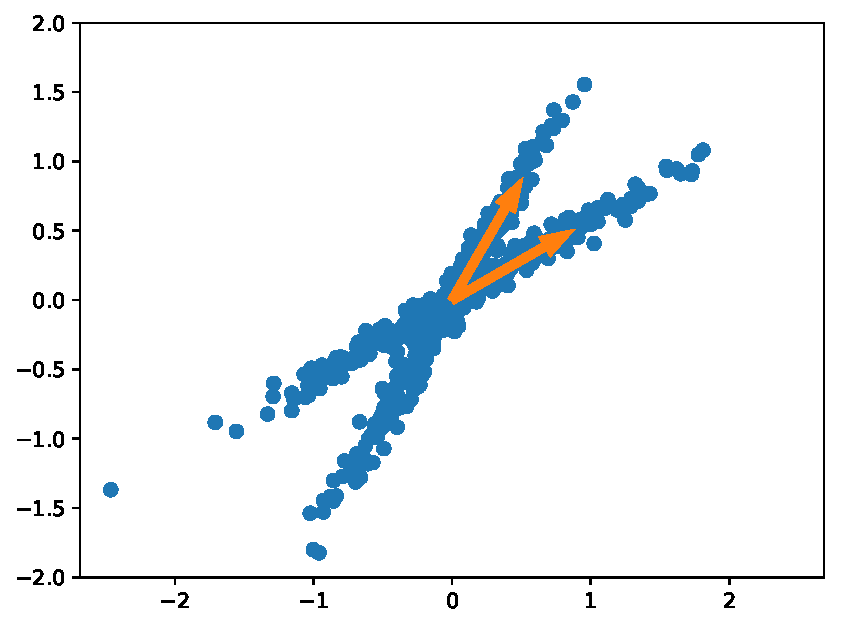
\includegraphics[width=\linewidth]{pca_opt1}
          \caption*{Option 1}
        \end{subfigure}%
        \begin{subfigure}{.33\textwidth}
          \centering
          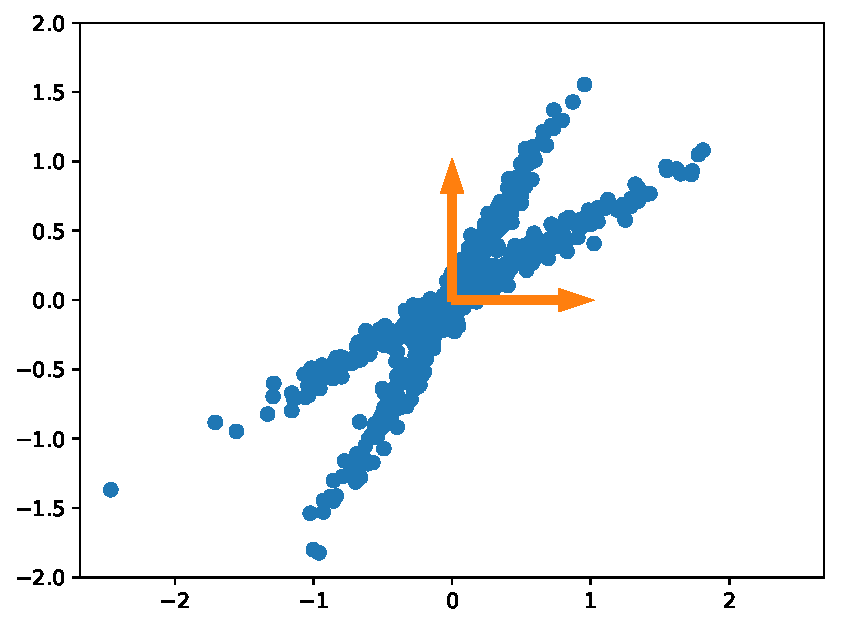
\includegraphics[width=\linewidth]{pca_opt2}
          \caption*{Option 2}
        \end{subfigure}%
        \begin{subfigure}{.33\textwidth}
          \centering
          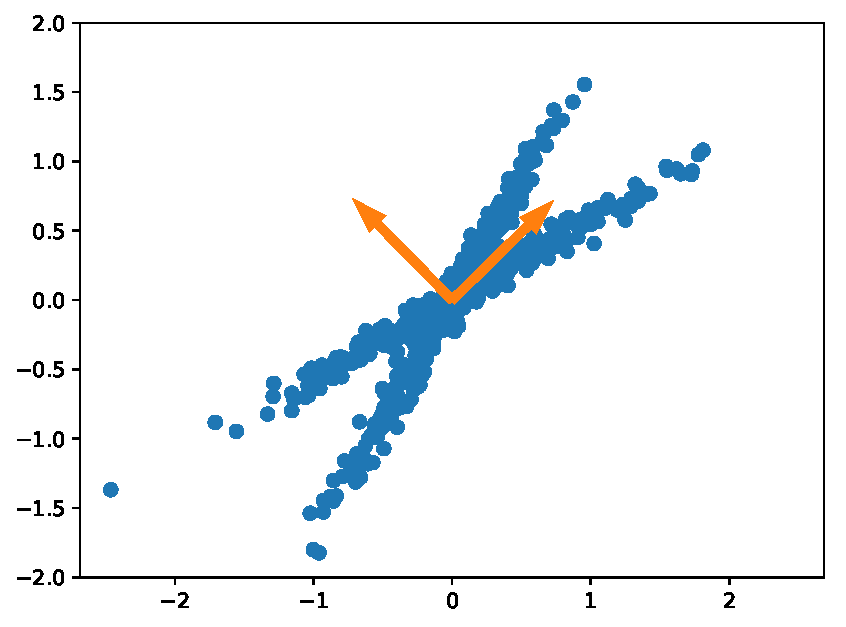
\includegraphics[width=\linewidth]{pca_opt3}
          \caption*{Option 3}
        \end{subfigure}
        \caption{Proposals of principal components on a 2D dataset}
        \label{fig:pca_proposal}
    \end{figure}
\item Consider the data in Figure~\ref{fig:pca_proposal}. Which of the following set of eigenvalues corresponds to the true principal components? Briefly explain your reasoning on each of the possible eigenvalue pairs.
    \begin{itemize}
        \item $l_1 = \begin{bmatrix}0.3\\0.3\end{bmatrix}$
        \item $l_2 = \begin{bmatrix}0.56\\0.04\end{bmatrix}$
        \item $l_3 = \begin{bmatrix}0.46\\-0.14\end{bmatrix}$
    \end{itemize}
    %\item Suppose we project the data from Figure~\ref{fig:pca_proposal} to the principal component with largest eigenvalue. How much of the data's variance will be explained by this projection?
\item Suppose we project the data from Figure~\ref{fig:pca_proposal} to the principal component with the largest eigenvalue. What will be the dimension of $\boldsymbol{W}$?
\end{enumerate}

\subsection{Singular Value Decomposition (SVD)}
In this exercise, we want to draw the connection between Singular Value Decomposition (SVD) and Principal Component Analysis (PCA). Let $\cxmat$ be the centered data matrix of size $N \times D$. SVD factorizes $\cxmat$ into three components $\cxmat = \boldsymbol{USV}^T$ where $\boldsymbol{U}$ is a $N \times N$ orthogonal matrix, $\boldsymbol{S}$ is a $N \times D$ rectangular diagonal matrix and $\boldsymbol{V}$ is a $D \times D$ orthogonal matrix. An orthogonal matrix $\boldsymbol{Q}$ has the property $\boldsymbol{Q}^T\boldsymbol{Q} = \boldsymbol{QQ}^T = \boldsymbol{I}$ where $\boldsymbol{I}$ is the identity matrix.

\begin{enumerate}[(a)]
    \item The sample covariance matrix $\boldsymbol{C}$ is given by $\boldsymbol{C} = \frac{\cxmat^T\cxmat}{N-1}$ where we apply element-wise division by the scalar $(N-1)$. Show that $\boldsymbol{C}$ can be decomposed as $\boldsymbol{C} = \boldsymbol{VLV}^T$ where $\boldsymbol{V}$ is the same orthogonal matrix as in the SVD of $\cxmat$.
    \item Using your result from (a), provide the expression for $\boldsymbol{L}$ (in terms of the decomposition factors of $\cxmat$). What is the dimension of $\boldsymbol{L}$?
    \item What are the eigenvectors and eigenvalues of $\boldsymbol{C}$? Hint: eigenvectors $\vvec$ and eigenvalues $\lambda$ of the matrix $\boldsymbol{A}$ satisfy the equation $\boldsymbol{A}\vvec_i = \lambda_i \vvec_i$
\end{enumerate}

\section{Chapter 7: Clustering}
For the next two problems, consider a dataset $\mathcal{X}_c=\{{\bf x}^i\}_{i=1}^N$ consisting of $N=5$  data-points.
The main goal of the next two problems is to cluster the dataset $\mathcal{X}_c$ reported in Figure~\ref{fig:clustering} into $k=2$ groups.

\begin{figure}[!ht]
	\centering
	\includegraphics[width=0.35\textwidth]{clustering_data.png}
	\caption{Visualization of the dataset $\mathcal{X}_c$.}
	\label{fig:clustering}
\end{figure}

\subsection{Agglomerative Hierarchical Clustering}
Given a measure of distance between clusters $d$, the procedure to perform agglomerative hierarchical clustering proceeds as follows:
\begin{itemize}
	\item  Initialize one cluster for each data-point
		\begin{align*}
			\mathcal{C}^i &= \left\{{\bf x}^i \right\}& \forall {\bf x}^i \in \mathcal{X}_c
		\end{align*}
	\item While the total number of clusters is greater then $k$
	\begin{enumerate}
		\item Compute the distance between each pair of clusters according to $d$
		\item Merge the two clusters $\mathcal{C}^i$ and $\mathcal{C}^j$ that have minimal distance
		\begin{align*}
			\mathcal{C}^{i,j} &= \mathcal{C}^i \cup \mathcal{C}^j
		\end{align*}
	\end{enumerate}
\end{itemize}
For this problem, $d$ will consider the minimum euclidean distance between the elements of the clusters.
More formally, given two clusters $\mathcal{C}^i$ and $\mathcal{C}^j$, the distance between them is defined as:
\begin{align}
	d(\mathcal{C}^i, \mathcal{C}^j) = \min \left\{ \|{\bf y}-{\bf z}\|_2 : {\bf y}\in\mathcal{C}^i, {\bf z}\in\mathcal{C}^j \right\}
	\label{eq:distance}
\end{align}
Where $\|{\bf y}-{\bf z}\|_2$ represents the euclidean distance between $\bf y$ and $\bf z$.
\begin{enumerate}[(a)]
	\item Perform agglomerative hierarchical clustering on the dataset $\mathcal{X}_c$ for $k=2$. Which data-points are part of the final two clusters? Show the iterative procedure by specifying which clusters are merged at each step.
	\item Consider a distance $d_2$ defined as the minimal squared euclidean distance between elements of two clusters:
	\begin{align*}
	d_{2}(\mathcal{C}^i, \mathcal{C}^j) = \min \left\{ \|{\bf y}-{\bf z}\|_2^2 : {\bf y}\in\mathcal{C}^i, {\bf z}\in\mathcal{C}^j \right\}
	\end{align*}
	What would change if we perform the clustering procedure considering $d_2$ instead of $d$? Justify your answer.
\end{enumerate}

\subsection{K-Means Clustering}
 For this problem, let $\bf b$ be an indicator vector for data point $\textbf{x}^i$ such that $b_{i} = 0$ if $\textbf{x}^i$ is a member of the first cluster and 1 if $\textbf{x}^i$ belongs to second one. Let $\textbf{m}_1$ and $\textbf{m}_2$ be the means of the two clusters respectively.
The most common form of the K-Means algorithm proceeds as follows

\begin{itemize}
\item {Initialize $\textbf{m}_1$ and $\textbf{m}_2$.}

\item Repeat the following two steps until the values of $\textbf{m}_1$ and $\textbf{m}_2$ are unchanged with respect to the previous iteration

\begin{enumerate}
\item Determine clusters for each sample $\textbf{x}^i$ by determining labels $b_i$.
\begin{align*}
b_i =
\begin{cases}
0,& ||\textbf{x}^i - \textbf{m}_1||^2 \le ||\textbf{x}^i - \textbf{m}_{2}||^2  \text{ i.e. $\textbf{x}^i$ belongs to cluster 1} \\
1, & \text{otherwise}
\end{cases}
\end{align*}

\item {Recompute $\textbf{m}_1$ and $\textbf{m}_2$ using the updates
	%Remove $j$ from $C$ if $\sum_{i=1}^n \gamma_{ij} = 0$. Otherwise, %
\begin{align*}
\textbf{m}_{1} &= \frac{\sum_{i=1}^N (1-b_i) \textbf{x}^i}{N-\sum_{i=1}^N b_i} & \textbf{m}_{2} &= \frac{\sum_{i=1}^N b_i \textbf{x}^i}{\sum_{i=1}^N b_i}
\end{align*}}

\end{enumerate}
\end{itemize}

\begin{enumerate}[(a)]

\item Perform the K-means clustering algorithm on the dataset $\mathcal{X}_c$ (Figure~\ref{fig:clustering}) by initializing ${\bf m}_1=\begin{bmatrix}2 \\ 3\end{bmatrix}$ and ${\bf m}_2=\begin{bmatrix}4\\2\end{bmatrix}$. Show each iteration of the algorithm by specifying the updates for the values of the assignments $\bf b$ and the means ${\bf m}_1$ and ${\bf m}_2$ until convergence.  

\item Repeat the K-means clustering algorithm by initializing ${\bf m}_1=\begin{bmatrix} 1 \\ 2 \end{bmatrix}$ and ${\bf m}_2=\begin{bmatrix} 3 \\ 3 \end{bmatrix}$ instead. Do we obtain the same result? Explain your findings.
\end{enumerate}


\section{Chapter 8: K-Nearest Neighbors}
For this problem we will consider a dataset $\mathcal{X}_k=\{{\bf x}^i\}_{i=1}^N$ consisting of $N=7$ data-points of two different classes. The goal of this exercise is to use the k-nearest neighbors algorithm to classify new observations. 
Figure~\ref{fig:knn} visualizes the examples $\{{\bf x}^i\}_{i=1}^N$ together with the instances ${\bf t}^1$ and ${\bf t}^2$ for which the label is unknown. 

\begin{figure}[!ht]
	\centering
	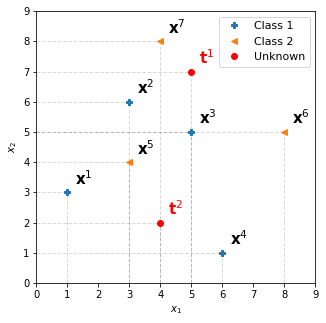
\includegraphics[width=0.5\textwidth]{k-nearest}
	\caption{Two-class dataset $\mathcal{X}_k$. 
}\label{fig:knn}
\end{figure}
In the most common version of the k-nearest neighbors algorithm, the class label of a new data-point is determined by the class assigned to the majority of its neighbors according to a specified distance measure. Answer the following questions:

\begin{enumerate}[(a)]
\item Consider the euclidean distance as the measure to determine the proximity of the data-points. Which is the class label associated to the test point ${\bf t}^1$ by considering $k=1$, $k=3$ and $k=5$ neighbors? Justify your answers by specifying the neighbors of ${\bf t}^1$ for the different values of $k$.
\item The cosine similarity is a popular measure to compare correspondences between vectors. Based on this notion, it is possible to define a measure of distance known as the cosine distance. Given two data-points ${\bf x}^i$ and ${\bf x}^j$, the cosine distance is defined as:
\begin{align*}
	d_{cos}({\bf x}^i,{\bf x}^j) = 1- \frac{({\bf x}^i)^T{\bf x}^j}{\|{\bf x}^i\|_2\|{\bf x}^j\|_2}
\end{align*}
By using the cosine distance to determine the neighbors, report the class label assigned to the test point ${\bf t}^2$ for $k=1$, $k=3$ and $k=5$. Specify the neighbors of ${\bf t}^2$ and its predicted label for each mentioned value of $k$.
\item What problem arises if we select $k=7$ to classify ${\bf t}^1$ and ${\bf t}^2$? Can we solve the problem by choosing a different distance metric? Explain your reasoning.

\end{enumerate}
\end{document}
